\appendix
\section{Appendix}
\label{app}

In this appendix, we provide additional details that, due to space
restrictions, could not be included in the main part of the paper. In
particular, this appendix covers the following aspects:
\begin{itemize}[noitemsep,left=1em]
\item A comparison of the query models adopted by different approaches for
event query discovery (\autoref{sec:languages}).
\item Additional experimental results on a comparison of our algorithms with
one that is based on representation learning (\autoref{sec:learning}).
\item A formalization of function \textsc{MergeAttributeQueries} to
merge queries found per attribute (\autoref{sec:alg_merge_attribute}).
\item A formalization of function \textsc{DescriptiveQueries} to select only
the descriptive queries in a set of queries
(\autoref{sec:alg_descriptive_queries}).
\item Formalizations of the D-U-S and B-S-S algorithms as instantiations of
the \sys{} framework (\autoref{sec:alg_further}).
\item A detailed discussion of completeness considerations for our
algorithms (\autoref{sec:completeness}).
\end{itemize}



\subsection{Query Model Comparison}
\label{sec:languages}

We first consider the query model adopted in iCEP~\cite{icep}. It is based
on an notion of events that are typed and carry a set of attribute values.
Queries are defined by operators that filter events, constrain their
attribute values, or require their joint or ordered occurrence, within a
certain time window.

Event query discovery with iCEP is organized in so-called learners, e.g.,
for learning the event types that are considered most relevant as they occur
in all given streams. However, considering the sequence learner to discover
an ordering of events, we note that it is applied solely on the level of
characterizations of events that have been derived in earlier steps. Such
characterizations correspond to query terms in our model. Hence, in
comparison to the algorithms of the \sys{} framework, iCEP is not capable to
discover queries that include the same query term multiple times. For the
database of our running example, see \autoref{ex1}, for instance, the query
$q_1 = \langle (\_,\text{schedule},\_),(\_,\text{schedule},\_)\rangle$
would not be discovered.

The IL-Miner~\cite{ilminer}, in turn, relies on an event and query model
that is close to the one underlying the \sys{} framework. That is, events
have a relational schema and queries define sequences of event variables,
which may be constrained by predicates. Such predicates may require an
attribute value of an event to assume a certain value, or they impose
correlation conditions by requiring the attribute values of two events to be
the same.

The discovery procedure of the IL-Miner first determines so-called relevant
event templates, i.e., sets of predicates that characterize relevant events.
Then, frequent sequence mining is used to extract an order over these
templates. While, this way, the above limitation discussed for iCEP is
avoided, the approach is also more restricted than our algorithms of the
\sys{} framework. In particular, the IL-Miner can only discover queries for
which the events are characterized by particular assignments of attribute
values. Hence, queries that only require the equivalence of attribute values
in events, but do not enforce any specific attribute values, cannot be
discovered. Again, using our example scenario from \autoref{ex1}, for
instance, it would be impossible to discover the query
$q_2 = \langle (\_,x_0,\_),(\_,x_0,\_)\rangle$.



\subsection{Comparison against a Representation Learning Approach}
\label{sec:learning}

To add another perspective, we report on experiments using a representation
learning algorithm for event streams, as introduced in~\cite{yanli2021}. The
approach learns a probabilistic
automaton to capture events and dependencies that indicate a situation of
interest. While the learned automaton is used for stream monitoring
in~\cite{yanli2021}, a query can be extracted from it by enumerating certain
transition paths~\cite{makowsky2012}. While this
approach
yields only type queries, no pattern queries or mixed queries, a comparison
sheds light on the potential of learning-based techniques for event query
discovery.


Since the algorithm can only discover type queries, we adapted one of our
algorithms (D-U-C) to also return only these queries.
This way, the outcome as well as the runtimes become comparable.
For the datasets F2b and G2b, \autoref{fig:rl} shows the obtained runtime
results, illustrating that our algorithm is at least two orders of magnitude
faster than the baseline algorithm. The effectiveness of query discovery is
summarized in \autoref{tab:rl_compare}. None of the descriptive queries is
discovered by the baseline (`Found'), while only one matching, but not
descriptive query is returned for either scenario (`$\neg$ Desc'). Also, the
construction based on representation learning yields several queries that
are not supported by the stream database (`$\neg$ Matching'). Hence, the
learning-based approach compromises correctness, descriptiveness, and
completeness and, due to high runtimes, is not suitable to address the
problem of
event query discovery.



\subsection{Merge Attribute Queries}
\label{sec:alg_merge_attribute}


\begin{figure}[t]
	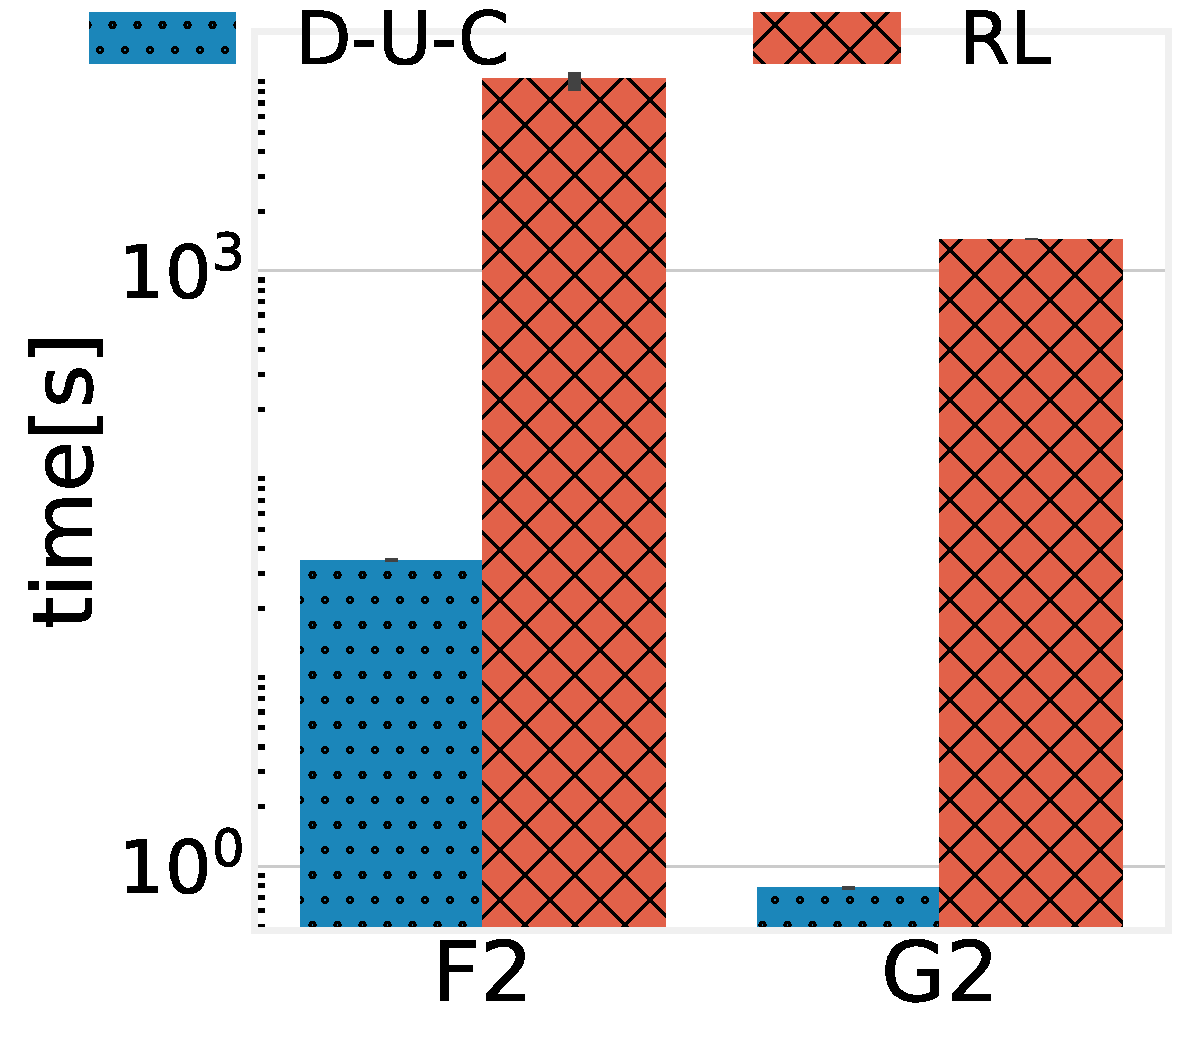
\includegraphics[width=0.45\columnwidth]{img/rl_compare.pdf}
	\vspace{-1em}
	\caption{Runtime, RL approach.}
	\label{fig:rl}
\end{figure}

\begin{table}[t]
	\footnotesize
	\caption{Comparison of our algorithms and the RL approach.}
	\vspace{-1em}
	\label{tab:rl_compare}
	\begin{tabular}{ccccc}
\toprule
Dataset & {Desc}(riptive) & Found & $\neg$ {Desc} & $\neg$
Matching\\
\midrule
F2b & 1 & 0 & 1 & 4 \\
G2b & 1 & 0 & 1 & 3 \\
\bottomrule
\end{tabular}

	%\vspace{-1em}
\end{table}


Our approach to merge queries found per attribute is defined as
\textsc{MergeAttributeQueries} in \autoref{alg-bu-df:mergedomainqueries}.
It takes as input a dictionary of matching queries for each attribute
$Q_{\mathcal{A}}: \mathcal{A} \rightarrow 2^{\mathcal{Q}}$, a parent
dictionary $P$, an event schema $\mathcal{A}$, a stream database $D$, and a
sequence of query variables $\mathcal{X}^<$; and returns a set of merged
queries.

In essence, the algorithm is based on an exhaustive combination of all
combinations of queries sourced from distinct attributes. Each resulting
combination then is handled in several steps:
\begin{itemize}
\item Instance Generation: Initially, for every query found for an
attribute, we systematically
generate all
feasible instances of the query within a single stream of the database.
\item Merge and Translation: Subsequently, we consolidate the instances of
the queries per attribute, and translate them into a unified query.
\item Query Matching: Following the merge, the obtained query is matched
against the stream database. If a match is identified, the merged query is
integrated into the result set.
\end{itemize}

\begin{algorithm}[t]
    \footnotesize
    \caption{\textsc{MergeAttributeQueries}}
    \label{alg-bu-df:mergedomainqueries}
    \KwIn{\, \ Dictionary of matching queries for each attribute
    	$Q_{\mathcal{A}}$,\\
    	\hspace{3em} \,  parent
    	dictionary $P$, event schema $\mathcal{A}$, stream database $D$,\\
    	\hspace{3em} \,  sequence of query variables $\mathcal{X}^<$.}
    %\tcc*{some comment}
    \KwOut{Set of descriptive queries $Q_d$.}
    \BlankLine
    % $n \leftarrow |\mathcal{A}|$\;
    $Q_{m} \leftarrow \emptyset$\;
    $\Gamma_D \gets \{a \in \Gamma \mid \forall \ S \in D: \exists \
	j\in\{1,...,|S|\}, i\in\{1,...,n\}: S[j].A_i = a\}$\;
	\tcc{\scriptsize{All combinations of queries from different
	attributes}}
    $L\leftarrow \bigtimes_{A\in\mathcal{A}}Q_{\mathcal{A}}(A)$\;
     \tcc{\scriptsize{Stream matches dictionary}}
    $T\leftarrow\emptyset$\;

    \ForEach{$(q_1,\ldots,q_n)\in L$}
    {
    		$I \gets \emptyset$\;
    		\lForEach{$q\in \{q_1,\ldots,q_n\}$}{$I(q) \gets \emptyset$}
	        \ForEach{$q \in (q_1,\ldots,q_n)$}
	        {
		\tcc{\scriptsize{Instance positions of query $q$ in $D$}}
		            $I(q) \leftarrow \textsc{GetInstances}(q,D)$\;
		  \If{$\forall q'\in \dom(P): P(q')\neq q $}{
                ${P \leftarrow}$
		\textsc{ChildQueries}($\mathit{q,\mathcal{A},\Gamma_D,P,\mathcal{X}^<,\True}$)\;
          }
          }
	        \tcc{\scriptsize{All
		combinations of instance positions of queries from different
		attributes}}
	        $B \leftarrow \bigtimes_{q_A\in\{q_1,\ldots,q_n\} } I(q_A)$\;
	        \ForEach{$(q'_1,\ldots,q'_n)\in B$}
	        {
	        	\tcc{\scriptsize{Translate instance tuple to query}}
		            $q_{m} \leftarrow
		            \textsc{Instance2Query}((q'_1,\ldots,q'_n),(q_1,\ldots,q_n))$\;
                    ${P \leftarrow}$
		\textsc{ChildQueries}($\mathit{q_m,\mathcal{A},\Gamma_D,P,\mathcal{X}^<,\True}$)\;
		            $q_p \leftarrow P(q_m)$\;
		            $M,T\leftarrow \textsc{Match}(q_m,\mathcal{A},
		            D,q_p,T)$\;
			    \tcc{\scriptsize{Add merged query to result set}}
		            \lIf{$M=\True$}
		            {
                   $Q_{m} \leftarrow Q_{m} \cup \{q_m\}$
			            }
		        }
	    }
    \Return $Q_m$\;
\end{algorithm}


\begin{algorithm}[t]
	\footnotesize
	\caption{\textsc{DescriptiveQueries}}
	\label{descriptivequeries}
	\KwIn{\, \ Set of queries $Q$, supported alphabet
		$\Gamma_D$, event schema $\mathcal{A}$,\\
		\hspace{3em} \,  sequence of query variables $\mathcal{X}^<$ over
		the set of query variables $\mathcal{X}$.}
	%\tcc*{some comment}
	\KwOut{Set of descriptive queries $Q_d$.}
	\BlankLine
	$Q_n\leftarrow \emptyset$\;
	\tcc{\scriptsize For each query $q$ in the query set $Q$, create queries
		which are less strict and therefore not descriptive}
	\ForEach{$q \in Q$}{
		$R \gets \emptyset$\;
		\lForEach{$s\in \Gamma_D\cup\mathcal{X}$}
		{$R(s)\gets \emptyset$}
		\ForEach{$i\in\{1,\dots,|q|\}$}{
			\label{alg10_1_start}
			\ForEach{$A\in\mathcal{A}$}{
				\If{$q[i].A \in \Gamma_D\cup\mathcal{X}$}
				{$q_n \gets q$\;
					$q_n[i].A \gets \_$\;
					$Q_n \gets Q_n\cup \textsc{Normalform}(q_n)$\;
					$R(q[i].A)\gets R(q[i].A)\cup \{i\} $\;
				}

			}
			\label{alg10_1_end}
		}
		\ForEach{$s\in\dom(R)$}{
			\If{$s\in\mathcal{X} \land |R(s)|\geq4$}{
				\label{alg10_2_start}
				\tcc{\scriptsize Find all combinations of partial
				replacements
					of variable $s$ in query $q$}
				$G\gets \textsc{GenerateReplacements}(q,s)$\;
				$Q_n \gets Q_n\cup G$\;
			}
			\label{alg10_2_end}
			\If{$s\in\Gamma_D \land |R(s)|\geq2$}
			{
				\label{alg10_3_start}
				\tcc{\scriptsize Find all combinations of partial and
				complete
					replacement of attribute type $s$ in query $q$}
				$G\gets \textsc{GenerateReplacements}(q,s)$\;
				% $q_n\gets q.\textsc{Replace}(s,x) |
				%x\in\mathcal{X}^<,R(x)=0$\;
				$Q_n \gets Q_n\cup G$\;
			}
			\label{alg10_3_end}
		}
	}
	$Q_d\leftarrow Q\backslash Q_n$\label{alg10_sub}\;
	\Return $Q_d$\;
\end{algorithm}

\subsection{Descriptive Queries}
\label{sec:alg_descriptive_queries}

Our approach to select only the descriptive queries in a set of queries is
given as \textsc{DescriptiveQueries} in \autoref{descriptivequeries}. Given
a set of queries $Q$, a supported alphabet
$\Gamma_D$, an event schema $\mathcal{A}$, and a sequence of query variables
$\mathcal{X}^<$ with $\mathcal{X}$ as the underlying set of query variables,
it proceeds as follows. We iterate over each
query $q$ within the given set and, for each query, generate queries that
are less specific than~$q$.
We generate less specific queries in three different ways:
\begin{itemize}
\item Replace each symbol (variable or attribute value) within the query by
the placeholder (\autoref{alg10_1_start}-\ref{alg10_1_end}). For every
replacement, a new non-descriptive query is added
to the set of non-descriptive queries $Q_n$.
\item Partially replace variables that appear at least four times within a
query by a new variable that is not used in query $q$
(\autoref{alg10_2_start}-\ref{alg10_2_end}).
\item Partially and completely replace attribute types that appear at least
twice within the given query  (\autoref{alg10_3_start}-\ref{alg10_3_end}).
\end{itemize}
At the end, we calculate the set of descriptive queries $Q_d$ by subtracting
all queries in $Q_n$ from the given set of queries $Q$ (\autoref{alg10_sub}).

The above approach relies on function \textsc{Normalform}, which checks, if
a variable occurs
at least twice, and otherwise replaces it with the placeholder $\_$. Second,
it restores the order of the variables, such that the first occurrences of
the variables appear in the same order in the query $q$ as they do in
$\mathcal{X}^<$.

%\examplebox{Example - Merging Attribute Queries}{
\begin{example}
	\label{ex:merge}
	Let us consider stream $S_2$ from \autoref{ex1}, the following queries
	per
	attribute, and their matching instances within the stream:



	\begin{center}
		\smallskip
		{\footnotesize
			\begin{tabular}{lll}
				\toprule
				Attribute & Query &  Positions \\
				\midrule
				Job Id & $\varepsilon, q_1=\langle (2,\_,\_) \rangle$   &
				$(e_{21})$, $(e_{23})$  \\
				Status   & $\varepsilon, q_2=\langle (\_,\text{schedule},\_)
				(\_,\text{schedule},\_) \rangle$ & $(e_{21}, e_{22})$   \\
				Priority   & $\varepsilon, q_3=\langle (\_,\_,\text{low})
				\rangle$ & $(e_{21})$, $(e_{23})$   \\
				\bottomrule
		\end{tabular}}
	\end{center}
	The combination of queries found for different attributes leads to the
	following set:
	$$\{(q_1,q_2,q_3), (q_1,q_2,\varepsilon), (q_1,\varepsilon,q_3),
	(\varepsilon,q_2,q_3),$$ $$(q_1,\varepsilon,\varepsilon),
	(\varepsilon,\varepsilon,q_3),
	(\varepsilon,q_2,\varepsilon),(\varepsilon,\varepsilon,\varepsilon)\}. $$
	The connection of the different position for the query tuple
	$(q_1,q_2,q_3)$ leads to the following merged queries:
	\begin{align*}
		&\langle (2,\text{schedule},\text{low}),(\_,\text{schedule},\_)
		\rangle \\
		&\langle
		(\_,\text{schedule},\_),(\_,\text{schedule},\_),(2,\_,\text{low})
		\rangle \\
		&\langle
		(2,\text{schedule},\_),(\_,\text{schedule},\_),(\_,\_,\text{low})
		\rangle \\
		&\langle
		(\_,\text{schedule},\text{low}),(\_,\text{schedule},\_),(2,\_,\_)
		\rangle
	\end{align*}
	which then have to be matched against the complete stream database.
	This process would have to be repeated for all combinations of query
	tuples to get all possible merged queries.
%}
\end{example}

Moreover, function \textsc{GenerateReplacements} takes as input a query $q$
and a symbol $s$, i.e., an attribute value or a variable that is to be
replaced by a variable, which is not used in the query.
The replacement routine first iterates through the number of symbols that can be replaced. In case of a variable (an attribute value) it is $[2,R(s)-2]$ ($[2,R(s)-1]$).
Then, for each group size, it finds all combinations of possible replacements for the current query $q$.

For example, let $s$ be a variable and $R(s)$=5. Let the positions of $s$
within the query be $[1,2,3,4,5]$.
Then the possible group sizes are 2 and 3.
For group size 2, there are $\binom{5}{2}=10$ combinations: $
(1,2),(1,3),\dots, (4,5)$.
For group size 3, there are $\binom{5}{3}=10$ combinations: $
(1,2,3),(1,2,4),\dots, (3,4,5)$.
For each of the calculated positions, $s$ is replaced by the same variable $x$ which is not
used in $q$.
The time complexity of the \textsc{GenerateReplacements} function is exponential,
$O(2^{R(s)})$, due to the generation of all combinations of replacements.
However, in practice, this complexity can be managed by typical constraints on
the values of $R(s)$ in the dataset and by applying optimizations to limit
the number of combinations generated.

The result is a set of
queries which are less specific than query $q$ and, therefore, not
descriptive.



\subsection{D-U-S \& B-S-S}
\label{sec:alg_further}

\sstitle{D-U-S: DFS, pattern-type unified, attribute separated}
As mentioned, the D-U-S algorithm, presented in \autoref{alg-bu-df-ds}, is a
variant of the D-U-C algorithm, which also
employs DFS and constructs queries in a unified manner.
It discovers queries separately per attribute, before merging
them to obtain the
final result. The sets of queries per attribute are maintained in a
dictionary $Q_{\mathcal{A}}: \mathcal{A} \rightarrow 2^{\mathcal{Q}}$, i.e.,
$Q_{\mathcal{A}}(A)$ is the set of queries found for attribute $A\in
\mathcal{A}$. The algorithm first constructs the projections of the streams
on the attribute (\autoref{alg9:projection}), which are then used to run the
D-U-C algorithm (\autoref{alg9:mining}). Note that setting flag $b$ to
$\False$ means that the D-U-C algorithm will return all found queries, not
only those that are descriptive. The queries discovered per attribute are
then merged, as detailed above, before the non-descriptive queries are
removed from the result.


\sstitle{B-S-S: BFS, pattern-type separated, attribute separated}
The B-S-S algorithm is defined in \autoref{alg-bu-bf-ds}. It is a variant of
B-S-C, adopting BFS and the separated
discovery of type queries and pattern queries. Yet, it first considers
queries per attribute, which are again collected in a
dictionary $Q_{\mathcal{A}}: \mathcal{A} \rightarrow 2^{\mathcal{Q}}$,
before merging them using the algorithm introduce above. As such, it
adopts the strategy explained above for D-U-S, just with B-S-C as the base
algorithm.



\begin{algorithm}[t]
	\footnotesize
	\caption{D-U-S}
	\label{alg-bu-df-ds}
	\KwIn{\, \ Stream database $D$, event schema $\mathcal{A}$, sequence of
		query var. $\mathcal{X}^<$.}
	\KwOut{Set of descriptive queries $Q$.}
	\BlankLine
	\tcc{\scriptsize Set of queries and parent dict. per
		attribute}
	$\mathit{Q_{\mathcal{A}}, P_{\mathcal{A}} \leftarrow \emptyset}$\;
	\ForEach{$A\in\mathcal{A}$}{$Q_{\mathcal{A}}(A), P_{\mathcal{A}}(A)
		\leftarrow \emptyset,\emptyset$\;}
	\tcc{\scriptsize Use D-U-C to discover queries per attribute}
	\ForEach{$A\in\mathcal{A}$}{
		\label{alg9:projection}
		$D_A \leftarrow \{\langle (e_1.A), \dots, (e_{l}.A)\rangle
		\mid \langle e_1,\ldots, e_l\rangle \in D \}$\;
		\label{alg9:mining}
		$Q_{\mathcal{A}}(A),P_{\mathcal{A}}(A)\leftarrow
		\textsc{D-U-C}(D_A,(A),\mathcal{X}^< ,\False)$\;
	}

	$P \leftarrow \cup_{A\in\mathcal{A}} P_\mathcal{A}(A)$\;
	\tcc{\scriptsize Merge queries found per attribute}
	$Q \leftarrow
	\textsc{MergeAttributeQueries}(Q_{\mathcal{A}},P,\mathcal{A},D,\mathcal{X}^<)$\;
	%%{\scriptsize \tcp*{\autoref{alg-bu-df:mergedomainqueries}}}
	$Q \leftarrow
	\textsc{DescriptiveQueries}(Q,\Gamma_D,\mathcal{A},\mathcal{X}^<)$\;
	%%{\scriptsize \tcp*{\autoref{alg-bu-df:mixedqueries}}}
	\Return $\mathit{Q}$\;
	%\textbf{break};
\end{algorithm}
\begin{algorithm}[t]
	\footnotesize
	\caption{B-S-S}
	\label{alg-bu-bf-ds}
	\KwIn{\, \ Stream database $D$, event schema $\mathcal{A}$, sequence of
	query var. $\mathcal{X}^<$.}
	\KwOut{Set of descriptive queries $Q$.}
	\BlankLine
	\tcc{\scriptsize Set of queries and parent dict. per
		attribute}
	$\mathit{Q_{\mathcal{A}}, P_{\mathcal{A}} \leftarrow \emptyset}$\;
	\ForEach{$A\in\mathcal{A}$}{$Q_{\mathcal{A}}(A), P_{\mathcal{A}}(A)
		\leftarrow \emptyset,\emptyset$\;}
	\tcc{\scriptsize Use B-S-C to discover queries per attribute}
	\ForEach{$A\in\mathcal{A}$}{
		\label{alg10:projection}
		$D_A \leftarrow \{\langle (e_1.A), \dots, (e_{l}.A)\rangle
		\mid \langle e_1,\ldots, e_l\rangle \in D \}$\;
		\label{alg10:mining}
	        $Q_{\mathcal{A}}(A),P_A\leftarrow
	\textsc{B-S-C}(D_A,(A),\mathcal{X}^< ,\False)$\;
	}

	$P \leftarrow \cup_{A\in\mathcal{A}} P_\mathcal{A}(A)$\;
	\tcc{\scriptsize Merge queries found per attribute}
	$Q \leftarrow
	\textsc{MergeAttributeQueries}(Q_{\mathcal{A}},P,\mathcal{A},D,\mathcal{X}^<)$\;
	%%{\scriptsize \tcp*{\autoref{alg-bu-df:mergedomainqueries}}}
	$Q \leftarrow
	\textsc{DescriptiveQueries}(Q,\Gamma_D,\mathcal{A},\mathcal{X}^<)$\;
	%%{\scriptsize \tcp*{\autoref{alg-bu-df:mixedqueries}}}
	\Return $\mathit{Q}$\;
\end{algorithm}


\subsection{Completeness}

\label{sec:completeness}
While we highlighted several arguments regarding completeness of our
algorithms already in \autoref{sec:realizations}, we now turn to a more
detailed discussion.
The functions that are relevant for an assessment of completeness, i.e.,
that determine that all potentially matching queries are generated at least
once to be checked for matching, are mainly: The algorithms for generating
query candidate, for merging pattern and type queries, and for merging
attribute queries.
We will discuss their completeness in dedicated subsections, i.e.,
\ref{sec:comp-candidates}, \ref{sec:comp-tp}, and \ref{sec:comp-att}.


\subsubsection{Query Candidate Generation}
\label{sec:comp-candidates}
Given a matching query (which, initially, is the empty query in all of our
discovery algorithms), new queries are generated following
a dedicated set of rules, which ensure that each potentially matching query
is generated exactly once:
\begin{enumerate}
	\item \textbf{New variables} are added to a query
	in two locations.  The first one concerns a placement after the first
	position of the last
	inserted variable. The second one concerns the position after the last
	inserted type.
	\item An \textbf{existing variable} is added to a query, only if this
	variable was
	the last inserted symbol. If this is the case, then it can be placed
	at any position after the last occurrence of this variable.
	\item A \textbf{new type} is added to the query  after the first
	position of the last inserted variable, or after the last position
	of any type.
\end{enumerate}
Recalling that the candidate generation always starts with the empty query,
it follows directly that all candidates can be generated based on the above
rules.

As such, the questions becomes if the above rules are correctly realized in
\autoref{alg-bu-df:childquery}. The three rules mentioned
above are implemented as follows: When inserting a new variable, first the
variable is instantiated.
Then, the algorithm iterates over each attribute. For each attribute,
we call the \textsc{Next}-Function which returns all helper queries
with possible first positions for the newly added variable. For all the
generated helper queries the \textsc{Next}-Function is called again
to determine the new candidate queries which are added to the
set of candidate queries.

To insert an existing variable again, we first check whether it
was the last inserted symbol.
Then, we determine the attribute of the variable and generate
new query candidates by calling the \textsc{Next}-Function.

Finally, to generate queries adding a new type, we again iterate
over all the attributes. For each attribute, we consider the
supported attribute values. For each supported attribute value,
the \textsc{Next}-Function is called, and the resulting queries
are added to the set of candidates.

The \textsc{Next}-Function iterates over the query terms starting
with the query term at position $s$ until the last query term of the query.
Then, per query term generates up to two new candidate queries:
First it checks whether the current attribute in the query term
is a placeholder. If this is the case, then it creates a new query
in which the current symbol is added to the attribute of the
current query term. Second it creates a new query by creating
a new query term right after the current one which only contains
the current symbol at the corresponding attribute and all the
other attributes are set as placeholders.



\subsubsection{Merge Pattern and Type Queries}
\label{sec:comp-tp}
To initalize the merging progress for all pairs of
type and pattern queries, for each of their parent queries $q$.
a 4-tuple is added to the queue of queries to be merged.
The 4-tuple consists of a type query $q_t$, a pattern or mixed query
$q_p$, a mixed query $q_m$ and an evolved query $q_e$. For the
initialization the tuple is set to
$(q_t, q_p, \langle\varepsilon\rangle, q)$
For each such tuple the function \textsc{MergeMixedQueries} is
called which is where the actual merging process takes place.

First the function calculates the starting position from which on
the mixed query can be extended.
If the evolved query is a type query then new merged queries are
generated by inserting the query term after the last occurence of another
type or attribute value,
adding each such generated query to the set of mixed queries.
It also checks whether the type to be added can be merged to an existing
query term in $q_m$.
If the evolved query is not a type query the function first checks
whether all query terms for either the type query or the pattern
query have already been incorporated into the mixed query.
If this is the case then starting from that position, the remaining
query terms of the eluded query are added to the end of the mixed query.
In a second step the function tries insert the current last position of
$q_p$ into the current query term of $q_m$. If this can be done
a new mixed query is generated which merges the query term and adds
the remaining query terms of the evolved query $q_e$.

For the 4-tuples created in the intialization
(\autoref{alg3:init_start}), The set of candidate queries
will either contain a type query
with one query term and one placed attribute value
(if $q_e$ is a type query) or $q_e$ if it is a pattern query.
The returned query candidates are matched and new
4-tuples are added to the queue accordingly.
For the initializiation tuples, the matching is obviously $\True$.
The next 4-tuples added to the queue are
$(q_e, q_p, q_n, q)$, where $q$ is either the empty query or one
of the parents of $q_p$ ($q_t$) if $q_e$ is a type query (pattern query).

Since $q_e$ is always a parent query we pass through all queries until
reaching the empty query.
This way it is assured that all possible queries are generated.


\subsubsection{Merge Attribute Queries}
\label{sec:comp-att}
The function first generates all combinations on $n$-tuples
for the matching attribute queries, such that in each $n$-tuple there
is a query from each attribute and $n$ being the number of
attributes. A valid query for each attribute is also the empty query.

For each $n$-tuple new possible mixed query candidates are generated
using the following procedure:
A function $I$ is called for each attribute query which returns
all the mappings of the query for each stream. For each stream
a list of $k$-tuples is returned, where $k$ is the number
of query terms for the current attribute query and each $k$-tuple
is a match of the query on that stream.

Then for one stream, we calculate all combinations of the different
$k$-tuples of the $n$ attribute queries. Each combination contains
one $k$-tuple from each attribute query in the current $n$-tuple.

It is sufficient to consider the instances of one stream, since
all matching queries necessarily need to match every stream.
This also means that only those queries present in one stream
are possible candidates to match the whole stream.

The resulting combinations of instance tuples are then
translated (if possible) to mixed queries and if they match
are added to the set of mixed queries.
